\documentclass[10pt,a4paper,titlepage,oneside]{article}
\usepackage{LabProtocol}

\exercise{Exercise II}

% enter your data here
\authors{
	Oliver Wöhrer, Matr. Nr. 11907563 \par
	{\small e11907563@student.tuwien.ac.at} \par
}


\begin{document}

\maketitle


%████████╗ █████╗ ███████╗██╗  ██╗     ██╗
%╚══██╔══╝██╔══██╗██╔════╝██║ ██╔╝    ███║
%   ██║   ███████║███████╗█████╔╝     ╚██║
%   ██║   ██╔══██║╚════██║██╔═██╗      ██║
%   ██║   ██║  ██║███████║██║  ██╗     ██║
%   ╚═╝   ╚═╝  ╚═╝╚══════╝╚═╝  ╚═╝     ╚═╝
\Task{VBS Graphics Controller}

\begin{qa}{VBS Oscilloscope Measurements}

	\begin{figure}[h!]
		\centering
		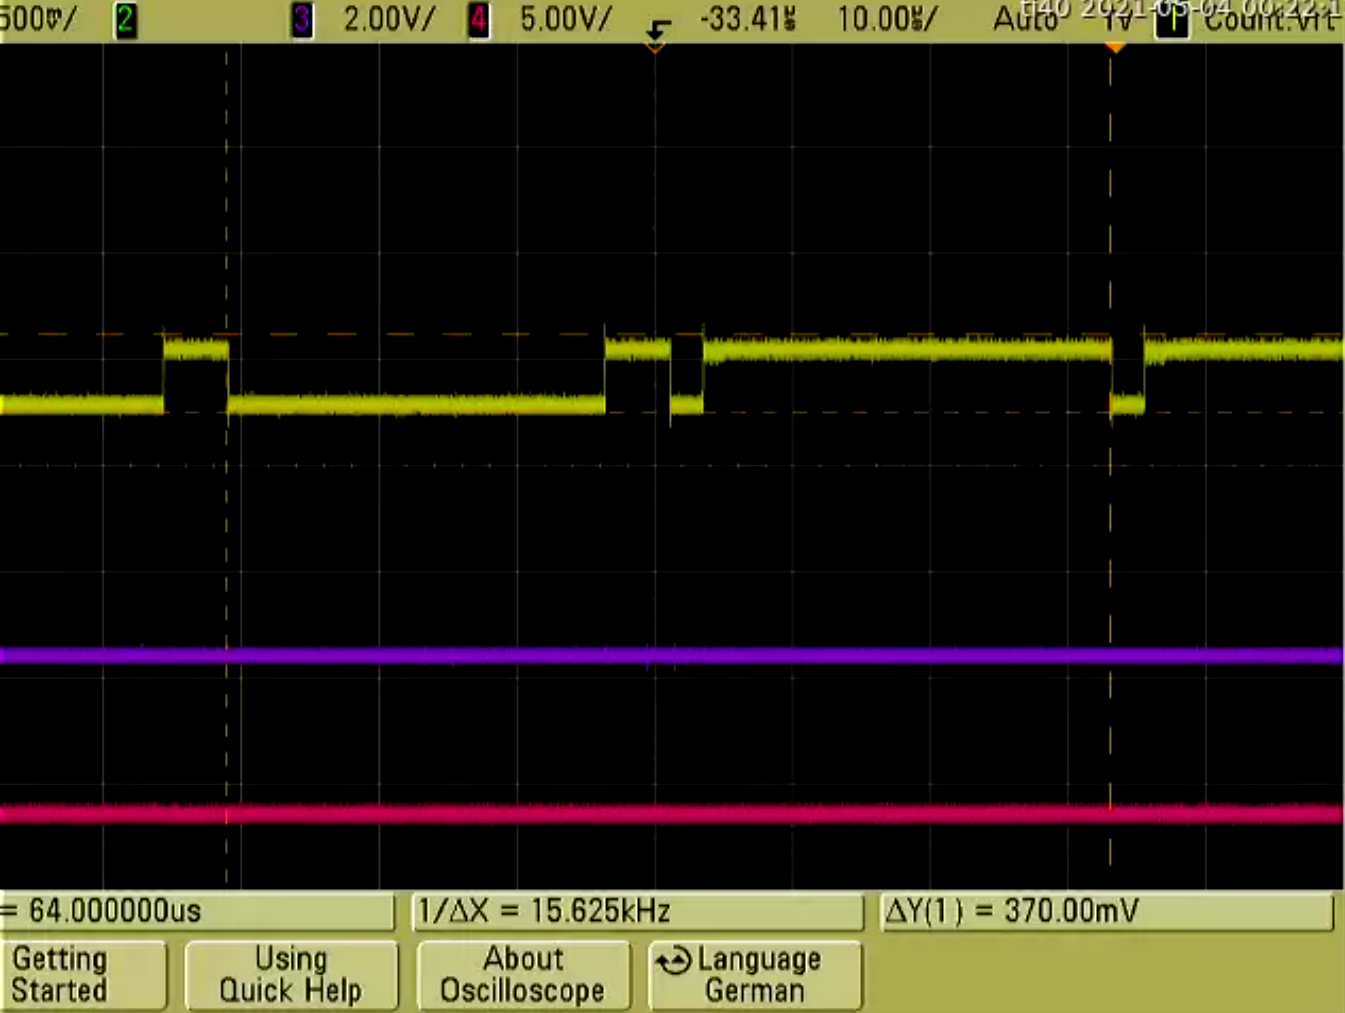
\includegraphics[width=1.0\linewidth]{dia/oszi_1_scanline3_timing.png}
		%\dummyimage
		\caption{Measurement showing scanline 3 with cursors marking the length (duration) of the whole line}
	\end{figure}
	
	\begin{figure}[h!]
		\centering
		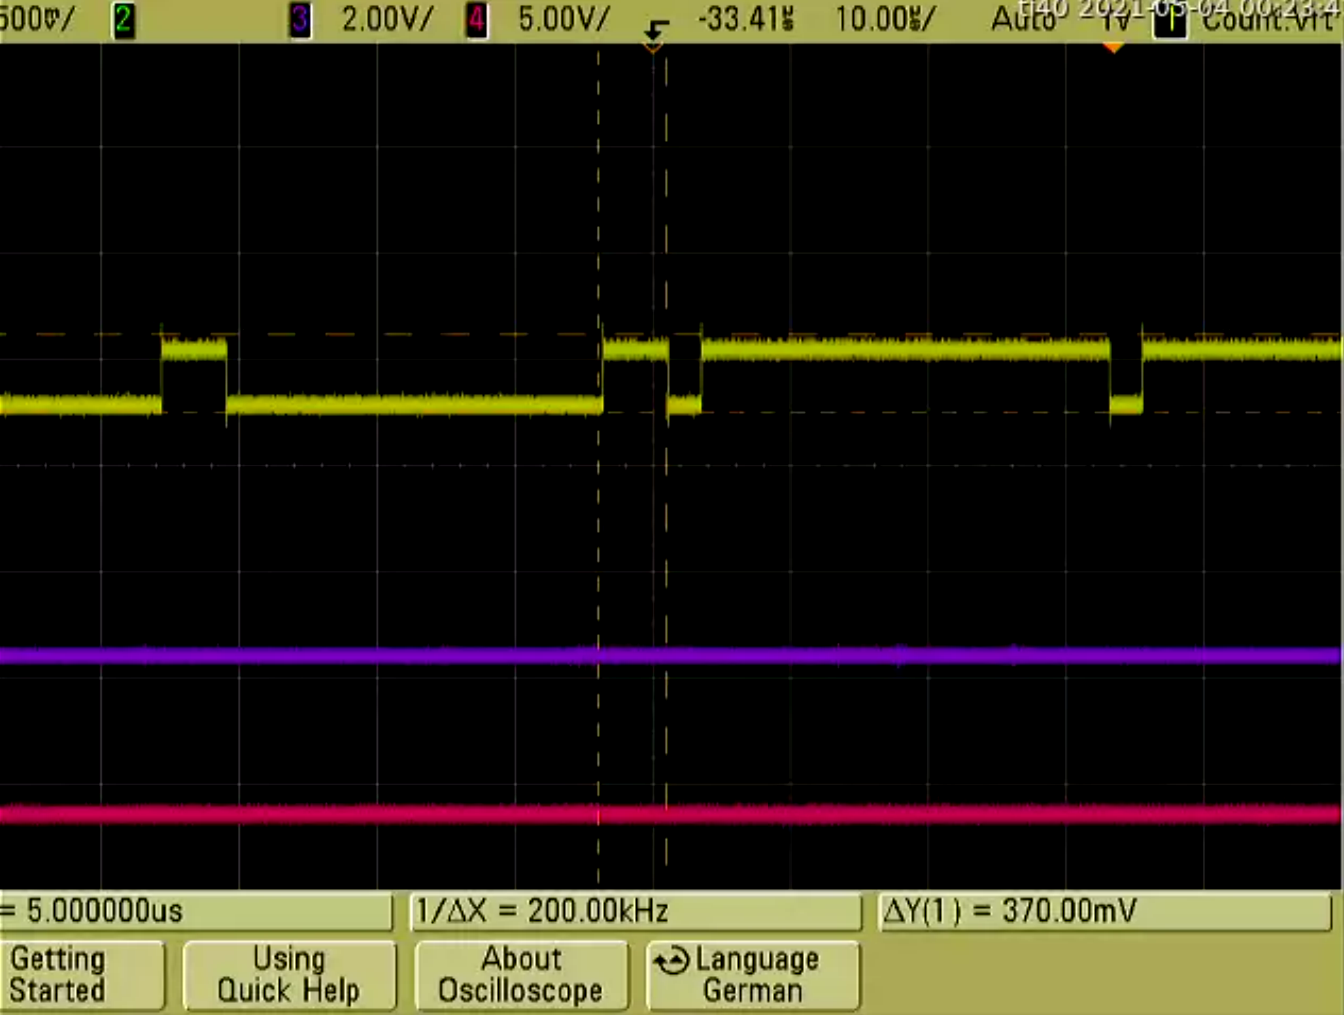
\includegraphics[width=1.0\linewidth]{dia/oszi_2_first_puls_1.png}
		%\dummyimage
		\caption{Measurement showing scanline 3 with cursors marking the duration of the first synchronization pulse}
	\end{figure}
	
	\begin{figure}[h!]
		\centering
		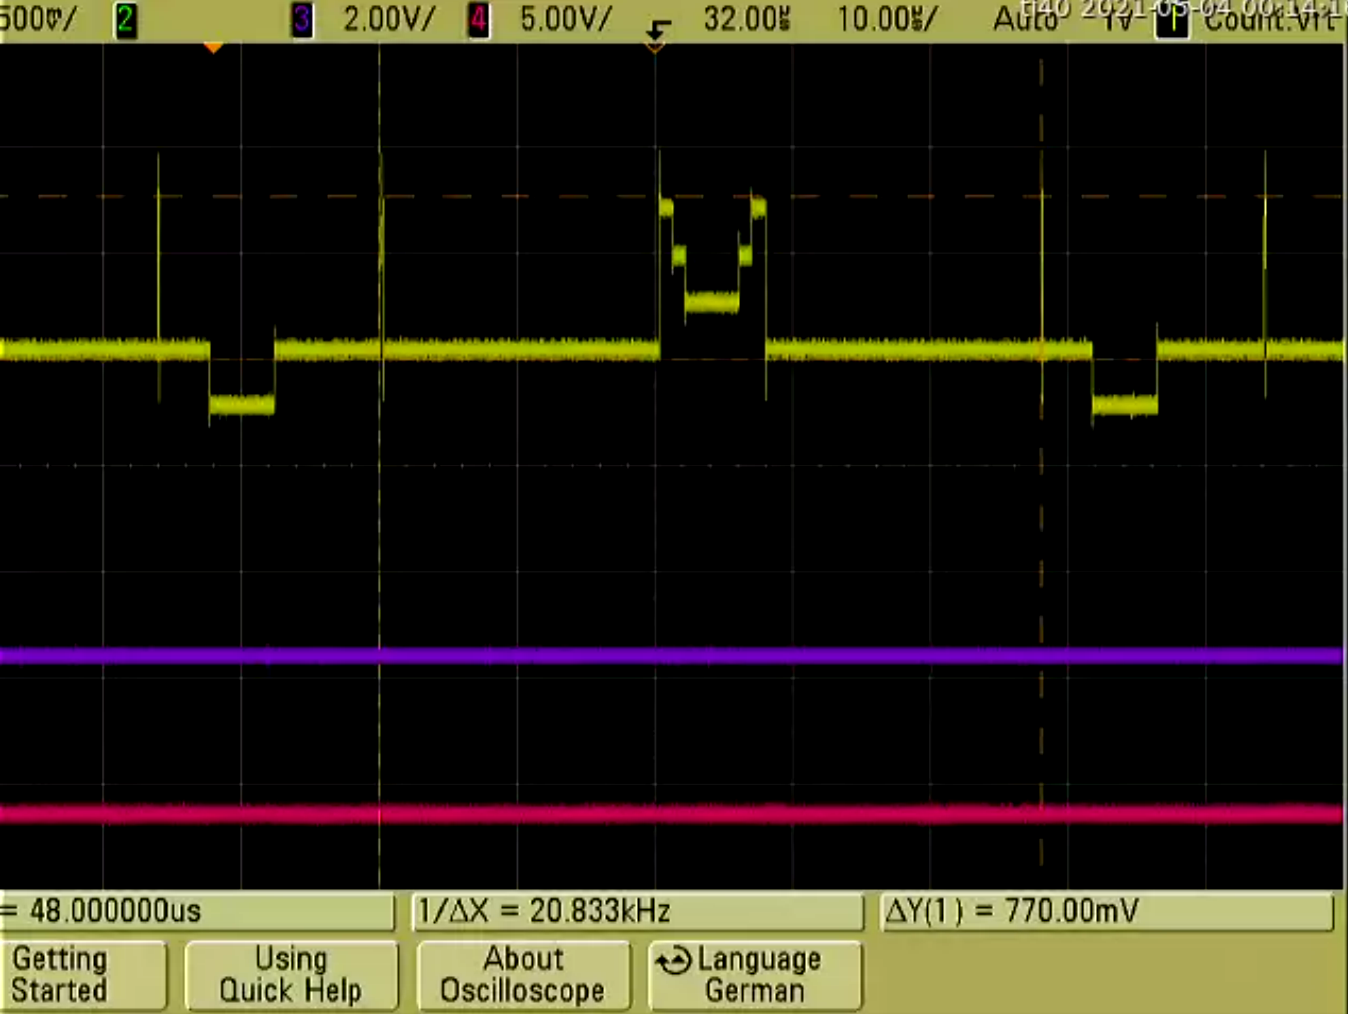
\includegraphics[width=1.0\linewidth]{dia/oszi_3_scanline160_levels.png}
		%\dummyimage
		\caption{Measurement showing a scanline of the center of the test pattern with cursors marking the visible portion of the line}
	\end{figure}

\end{qa}
%%%%%%%%%%%%%%%%%%%%%%%%%%%%%%%%%%%%%%%%%%%%%%%%%%%%%%%%%%%%%%%%%%%%%%%%%%%%%%%%


%████████╗ █████╗ ███████╗██╗  ██╗    ██████╗ 
%╚══██╔══╝██╔══██╗██╔════╝██║ ██╔╝    ╚════██╗
%   ██║   ███████║███████╗█████╔╝      █████╔╝
%   ██║   ██╔══██║╚════██║██╔═██╗     ██╔═══╝ 
%   ██║   ██║  ██║███████║██║  ██╗    ███████╗
%   ╚═╝   ╚═╝  ╚═╝╚══════╝╚═╝  ╚═╝    ╚══════╝
\Task{Ball Game module}

\begin{qa}{Briefly describe the architecture of your \textsf{ball\_game} module. Are there any submodules? What is their purpose? How many FSMs did you use?}
add your explanation here (approximately 8-10 sentences, you can also include figures) ... 
\end{qa}
%%%%%%%%%%%%%%%%%%%%%%%%%%%%%%%%%%%%%%%%%%%%%%%%%%%%%%%%%%%%%%%%%%%%%%%%%%%%%%%%

%████████╗ █████╗ ███████╗██╗  ██╗    ██████╗ 
%╚══██╔══╝██╔══██╗██╔════╝██║ ██╔╝    ╚════██╗
%   ██║   ███████║███████╗█████╔╝      █████╔╝
%   ██║   ██╔══██║╚════██║██╔═██╗      ╚═══██╗
%   ██║   ██║  ██║███████║██║  ██╗    ██████╔╝
%   ╚═╝   ╚═╝  ╚═╝╚══════╝╚═╝  ╚═╝    ╚═════╝ 
\Task{Bonus: SignalTap Measurement}

\begin{qa}{Trigger Condition}
	\begin{figure}[h!]
		\centering
		% \includegraphics[width=1.0\linewidth]{your filename here}
		\dummyimage
		\caption{Screenshot showing the trigger condition }
	\end{figure}
\end{qa}
%%%%%%%%%%%%%%%%%%%%%%%%%%%%%%%%%%%%%%%%%%%%%%%%%%%%%%%%%%%%%%%%%%%%%%%%%%%%%%%%

\begin{qa}{Measurement Screenshot}
	\begin{figure}[h!]
		\centering
		% \includegraphics[width=1.0\linewidth]{your filename here}
		\dummyimage
		\caption{Screenshot showing at least the first 4 instructions (and their associated data items) issued to the graphics controller during one frame by the \textsf{ball\_game} module.}
	\end{figure}
\end{qa}
%%%%%%%%%%%%%%%%%%%%%%%%%%%%%%%%%%%%%%%%%%%%%%%%%%%%%%%%%%%%%%%%%%%%%%%%%%%%%%%%

\begin{qa}{Instruction Decoding}
	\begin{center}
	\scriptsize
	\begin{tabular}{p{0.05\linewidth}p{0.2\linewidth}p{0.25\linewidth}p{0.40\linewidth}}
		\textsf{gfx\_instr} & associated \textsf{gfx\_data} items      & Instruction    & Description \\\hline\hline
		0x..                & \valuelist{0x0001,0x0002,0x0003,0x0004}  & GFX\_INSTR\_?? & ...\\\hline
		0x..                & \valuelist{0x0001,0x0002,0x0003,0x0004}  & GFX\_INSTR\_?? & ...\\\hline
		0x..                & \valuelist{0x0001,0x0002,0x0003,0x0004}  & GFX\_INSTR\_?? & ...\\\hline
		0x..                & \valuelist{0x0001,0x0002,0x0003,0x0004}  & GFX\_INSTR\_?? & ...\\\hline
	\end{tabular}
	\end{center}
\end{qa}
%%%%%%%%%%%%%%%%%%%%%%%%%%%%%%%%%%%%%%%%%%%%%%%%%%%%%%%%%%%%%%%%%%%%%%%%%%%%%%%%

\begin{qa}{What resources on the FPGA and board do you need to perform a measurement with a stand-alone logic analyzer (LA) measurement device and what for the SignalTap LA?}
put your answer here ... 
\end{qa}
%%%%%%%%%%%%%%%%%%%%%%%%%%%%%%%%%%%%%%%%%%%%%%%%%%%%%%%%%%%%%%%%%%%%%%%%%%%%%%%%
\end{document}
